\documentclass[12pt]{report}

\usepackage{graphicx}
\usepackage{textcomp}
\usepackage[margin=1.0in]{geometry}
\usepackage[symbol]{footmisc} % Used to have symbols for footnotes instead of numbers (so as to not get confused between references and footnotes)
\usepackage{gensymb} % Used for the degree symbol in math mode
\usepackage[subrefformat=parens,labelformat=parens]{subfig} % Used to combine figures into one
\usepackage{cleveref} % Makes references easier
\usepackage{bm} % Used for bold font in math mode
\usepackage[superscript,biblabel,sort]{cite} % The superscript option puts the references as superscript numbers, biblabel applies the superscript to the references page, and sort sorts the numbers from least to greatest, and if possible, puts a dash to shorten it (i.e. 1,2,3,4,5,6 will be shortened to 1-6)
\usepackage{wrapfig}

\bibliographystyle{aip2}

% This is the Introduction and Background section of the paper
\begin{document}
\begin{wrapfigure}{r}{0.4\textwidth}
%\begin{figure}[ht!]
\vspace{-20pt}
\centering
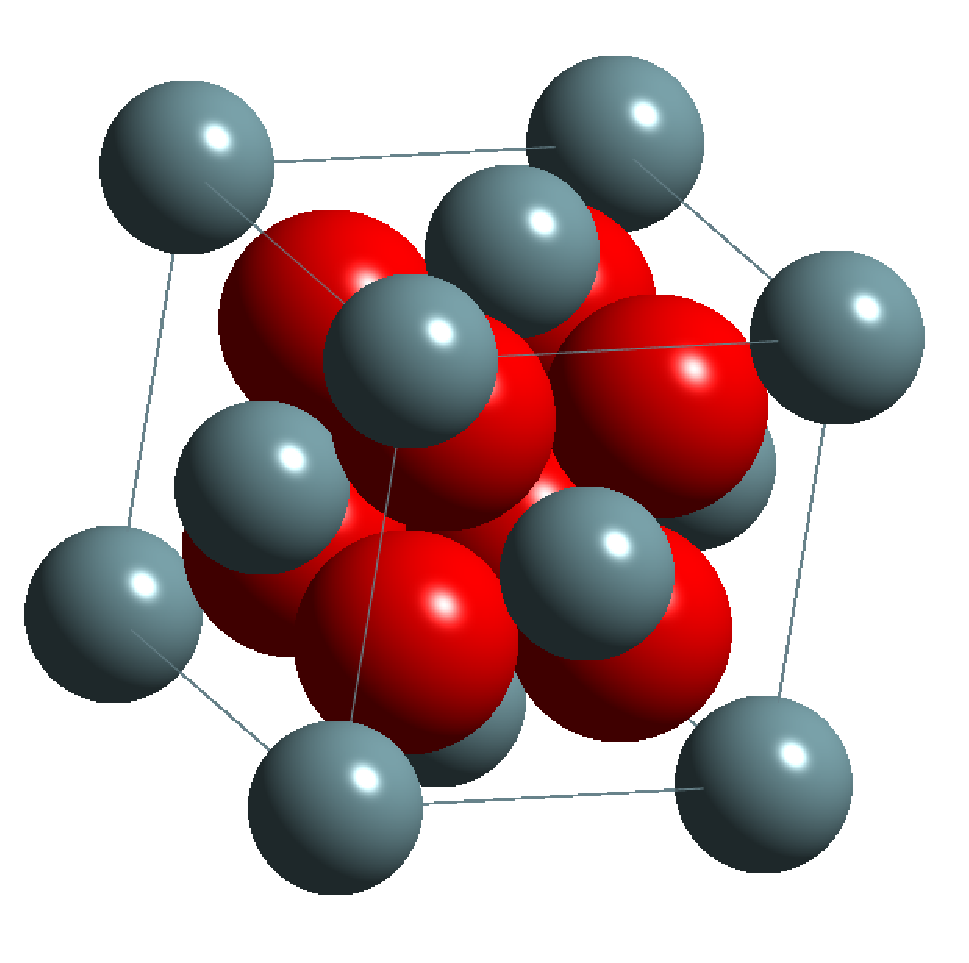
\includegraphics[scale=0.7]{Images/UO2}
\vspace{-10pt}
\caption[Example of the fluorite crystal structure.]{\label{fig:uo2Lattice}An image representing the fluorite crystal structure.  For UO\textsubscript{2}, the smaller spheres indicate the uranium atoms, and the larger spheres indicate the oxygen atoms.  Image courtesy of the University of Cambridge under the Creative Commons license.}
\vspace{-10pt}
%\end{figure}
\end{wrapfigure}
Uranium dioxide (UO\textsubscript{2}) is the primary choice for nuclear fuel in today's reactors.\cite{uraniumInfo}  Understanding the properties of UO\textsubscript{2} requires an analysis of the basic crystal structure of the material.  UO\textsubscript{2} is a ceramic (a type of polycrystalline material), meaning that a series of crystal lattices join together in various ways (called twist, tilt, or mixed boundaries) to create it.  This material has a fluorite crystal structure, where the uranium atoms form a face-centered cubic (fcc) lattice, and the oxygen atoms form a simple cubic lattice within the fcc frame (see \Cref{fig:uo2Lattice}).

The various properties of the fuel need to be well understood to make running the reactor as safe and effective as possible.  Some of these properties include thermal conductivity (how well heat flows through the material), fission gas release (how some of the fission products move throughout the material as gases), and mechanical stability (i.e. how the material bends or cracks under pressure or heat).  Taking thermal conductivity as an example, knowledge of this material property allows the most effective use of coolant to keep the reactor within operating temperatures, maximizing both efficiency and safety.  Knowledge of other material properties allows for similar gains in efficiency, safety, or both.

Interest in understanding UO\textsubscript{2} while in-reactor has led to efforts to more deeply understand the properties of the material.  Currently, Idaho National Laboratory (INL) faces the challenge of not having a completely accurate model of grain boundary energy anisotropy.  The current model assumes an isotropic energy, and this leads to an inability to model the material parameters correctly while in-reactor.  This in turn makes efforts in nuclear energy less efficient and/or safe than it otherwise could be.  INL aims to accurately model nuclear fuel while in-reactor, allowing accurate predictions regarding how the material properties will change.

This work adds to the safety and efficiency of using nuclear energy by providing the necessary information to accurately calculate the material properties of UO\textsubscript{2} in-reactor.  Specifically, this work improves the fitting parameters for grain boundary (GB) energy interpolation for UO\textsubscript{2} by using molecular dynamics (MD) results calculated by Zhang\cite{zhang2016} and Hansen\cite{hansen2016} with an anneal of 800 K.  Furthermore, this work begins preliminary efforts towards using more accurate functions to describe GB energy behavior.  Previous data did not use annealed crystal structures\cite{harbison2015}, which prevented the atoms from finding their ideal energetic minimum.  The 800 K anneal allows the atoms to relax to a value closer to their global minimum, as shown in \Cref{results}.  A database will store these simulated energies, and a MATLAB\textsuperscript{\textregistered} script will use the database to fit the function parameters.  INL will incorporate the updated parameters into its mesoscale phase field modeling platform MARMOT for use in modeling nuclear fuels.  As the modeling software incorporates these parameters, various tests of the UO\textsubscript{2} fuel can determine how the material properties change while in-reactor.

\chapter{Background\label{background}}
Polycrystalline materials (ceramics, metals, and polymers) are composed of tiny crystals called \emph{grains}.  The orientation of each grain does not generally depend on the orientation of the surrounding grains. Therefore, depending on how the crystal formed,\cite{callister2003} the crystal structures will possibly not line up at the interfaces where two grains meet.  This ``atomic mismatch"\cite{callister2003} leads to broken or stretched atomic bonds where atoms will not line up relative to a perfect crystal structure.  These defects are called grain boundaries (GBs, see \Cref{fig:gb}). The most popular way to parameterize a GB uses the five degree-of-freedom (DoF) model.\cite{patala2013, lejcek2010, homer2015, bulatov2014, harbison2015, rohrer2011}.  This model only uses the macroscopic DoFs (the observable DoFs corresponding to the misorientation and inclination), ignoring the three translational DoFs (the ability of the grain to move or slide anywhere in space) possessed by each grain.  Three of the five DoFs specify the misorientation (or misaligment) of the grains with respect to each other.  The other two DoFs specify the orientation of the grain boundary plane (called the inclination).  The rotation axis and angle define the misorientation DoFs, and the GB normal defines the inclination DoFs.\cite{lejcek2010}

Three specific types of GBs occur in polycrystalline materials: twist, tilt, and mixed GBs.\cite{lejcek2010, rohrer2011}  These GBs desribe the misorientation of two grains with respect to each other.  Twist boundaries have the axis of rotation between the two grains and the GB normal parallel to each other. Tilt boundaries can be either symmetric or asymmetric.  A perpendicular relationship between the axis of rotation between two grains and the GB normal creates a tilt boundary.  Symmetric tilt boundaries describe a GB whose boundary plane is a mirror plane: the atoms on one side of the boundary plane mirror the other side.  This makes the angles between the boundary plane and the orientation axes of the two grains equal. Asymmetric tilt boundaries have unequal angles.  \Cref{fig:misorientation} shows a representation of tilt boundaries (top) and twist boundaries (bottom).  A mixed GB combines twist and tilt boundary characteristics.

\begin{figure}[ht!]
\vspace{-20pt}
 \centering
 
 \subfloat[]{\label{fig:gb}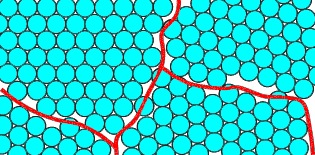
\includegraphics[scale=.9]{Images/grainBoundary}}\quad
 \subfloat[]{\label{fig:misorientation}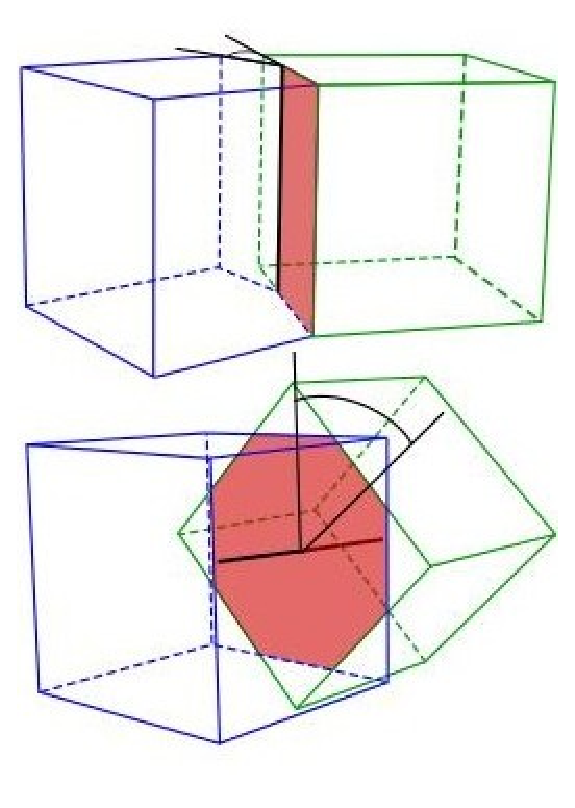
\includegraphics[scale=.6]{Images/twistTilt}}\quad
 \caption[Examples and types of grain boundaries.]{\label{gbs} A representation of GBs, where \protect\subref{fig:gb} shows an example of a grain boundary and \protect\subref{fig:misorientation} shows an example of GB types.  In \protect\subref{fig:gb} circles represent individual atoms of the grains, and the line represents the grain boundary.  Atomic mismatch between the differently oriented grains causes an excess of energy within the material, which has an effect on the material's properties.  Image courtesy of the University of Cambridge under the Creative Commons license. In \protect\subref{fig:misorientation} the tilt GB (top) has a perpendicular relationship between the axis of rotation and the GB normal, while the twist GB (bottom) has a parallel relationship between the two.  Image courtesy of Wikipedia under the Creative Commons license.}
\end{figure}

GBs have various effects on material properties, making them important to understand.\cite{patala2013, homer2015, bulatov2014}  The crystal structure has extra energy because of the atomic mismatch at the boundaries.  This extra energy, called GB energy, gives rise to GB motion.  Knowing and predicting how the GBs will move allows for more accurate calculations of a material's properties.  Thus, GB energy needs to be understood to accurately model the evolution of material properties.

Two methods of modeling GB energy are the isotropic and anisotropic models.  The most common method (and easier method) is the isotropic model.  This model ignores the impact of inclination on the GB energy, and assumes equal inclinations for a given misorientation, reducing the five-dimensional (5D) parameter space to a three-dimensional (3D) parameter space.  The reasons for assuming this model historically were based on the assumption that the inclination had little or no impact on the GB energy, or (later) that it was too difficult to create a full five DoF model.\cite{homer2015}  Alternatively, the anisotropic approach seeks to quantify the effect that misorientation \emph{and} inclination have on the GB energy.  Currently, researchers acknowledge the need for a full five DoF model of GB energy, but assert the difficulty inherent in developing such a model.\cite{rohrer2011, lejcek2010, homer2015}  Despite these difficulties, GB energy functions for certain materials, namely fcc metals copper, gold, aluminum, and nickel, have proven successful.\cite{bulatov2014} Recently,\cite{harbison2015} similar efforts created a GB energy function for ceramics.  This work improves the accuracy of the energy interpolation function for UO\textsubscript{2}.

\bibliography{gbCharacter}
\end{document}